\section[Flexible Standards]{Aim 1 - Flexible Standards for categories definition}

The measure of retention of patients under \gls{art} is a key measure of HIV programs performance. HIV being a chronic disease, the measure of success of these treatments is indeed the survival of treated patients, which is directly dependent to their adherence to \gls{art} treatment. As HIV programs have been rolled out in different countries, the importance of \gls{ltfu} in \gls{art} cohorts has been recognized, and since the early days of HIV care programs, efforts have been made to better measure and understand the how and why patients remain in care on the long term   \citep{ioannidis_predictors_1999,lebouche_incidence_2006,moh_incidence_2007}.

Initiating treatment programs, HIV practitioners used the categories that had been developed and used in clinical trials to categorize patients outcome. This definition is mainly a negative category, grouping patients who failed to attend their medical appointments and for which no definitive had been recorded. \gls{ltfu} is thus defined by an absence of data about a patient more than by a positive element of information.

As HIV programs were rolled out, it soon became clear that the \gls{ltfu} category, in many settings, is a mixed bag of patients with different status \citep{kwong-leung_yu_true_2007,dalal_characteristics_2008,mcguire_vital_2010}. This poses problems for HIV programs evaluation, as the true outcome of HIV patient is often unknown, and different authors have proposed ways to correct retention measures by collecting additional data
 \citep{yiannoutsos_sampling-based_2008,geng_tracking_2010,tassie_evaluation_2010}, or by fitting correcting models \citep{brinkhof_adjusting_2010,egger_correcting_2011,van_cutsem_correcting_2011,henriques_comparison_2012,verguet_incorporating_2013}.
Finally, some authors started paying attention to how the very metric used to measure patients retention could heavily impact the evaluation of HIV programs performance \citep{chi_empirical_2010,chi_universal_2011,fox_defining_2012,mugavero_measuring_2012,yehia_comparing_2012,grimsrud_impact_2013,shepherd_impact_2013}.

An important underlying hypothesis of the use of the \gls{ltfu} metric as a proxy for retention is that, if the patient had been coming to the facility for an appointment, this visit would have been recorded. This hypothesis makes sense considering the notion of \gls{ltfu} comes from the clinical trial setting \citep{lebouche_incidence_2006} but it can be problematic in developing countries, where data quality in care setting is often difficult to guarantee. In these settings, the delay between a visit and the time of data entry will be important, mechanically inflating the number of \gls{ltfu} \citep{lurton_report_2012}. There is thus an equivalence established between patient's status and data quality in the facility. Meanwhile, assessing data quality of a database and its impact on the measure of retention is seldom made.

With the development and rollout of \gls{emr} in facilities, there is an opportunity to improve on this situation. Most computerized data collection systems collect metadata on data entry, such as the date at which a form was entered, or the role of the person doing the data entry. This metadata could be mobilized to measure the quality of the data, and to understand the impact of data quality on the measure of retention.

This project main aim is to simulate and describe the impact of data quality on the measure of retention of patients in HIV cohorts. This will be achieved through three specific aims :

\begin{description}
	\item[Impact of data quality on the measure of retention] I will model the path through which data quality impacts the measure of retention, and will simulate the results metrics of an HIV cohort with varying data quality.
	\item[Data Maturity] As the time to data entry is an essential element of data quality and directly impacts the measure of retention, the ability to properly measure retention for a given period improves over time. I will define a metric of data maturity to describe the ability of a database to measure retention for a cohort. This measure will be tested and validated on the simulated cohort.
	\item[Robust Retention Metrics] Building on the insights gained in the previous aims, I will define, test and validate different robust retention metrics for HIV cohorts. These metrics will be evaluated on their ability to properly measure the retention of patients in a simulated cohort, and on their robustness to varying data quality.
\end{description}


\subsection{Theoretical Framework}

\subsubsection{HIV care process}

HIV patients are visiting hospitals for regular appointments. At each visit, they are given an appointment for their next visit. The date for the $v^{th}$ visit of patient $i$ is noted $V_v^i$, and the appointment time for this visit is noted $A_v^i$. Thus, if $V_v^i > A_v^i$, the patient came late to his appointment, if $V_v^i < A_v^i$, the patient came early. We note $l_v^i = A_v^i - V_v^i$, the lag between scheduled appointment and actual visit. Figure \ref{fig:late_days} shows the distribution of $l_v^i$ in our data. Unrecorded appointments are handled by dividing the time between scheduled appointment and actual visit by 28, and considering the remainder. The spikes around 7, 14 and 21 days show either patients who were given an unrecorded appointment of less than a month, or is proof to the fact that patients have favorite days of visit.

\begin{center}
\begin{figure}[ht]
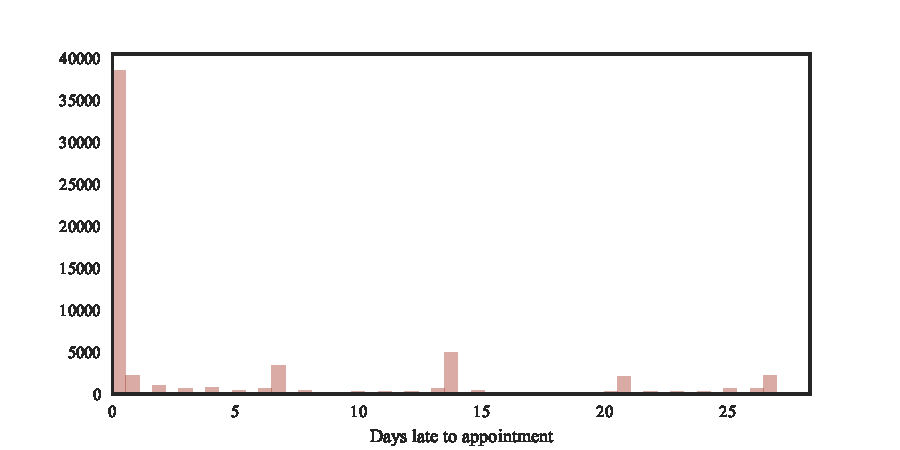
\includegraphics[width=\textwidth]{figure/time_late_to_appointment.pdf}
\caption{Distribution of $l_v^i$ in our data.}
\label{fig:late_days}
\end{figure}
\end{center}

The time elapsed between a visit and the next scheduled appointment is set by the national norms regarding the frequency at which HIV patients should be evaluated, depending on their condition and medical history. Patients recently enrolled in care will be seen more frequently than patients with a longer follow-up and no complications. We note ($f_v^i$) the visit frequency regimen of patient $i$ at visit $v$. This unit is usually around a multiple of 28 days, as patients are likely to have a favorite week day for visit (cf. \textit{supra}). Figure \ref{fig:schedule_days} shows the distribution of $f_v^i$ in our data.

\begin{center}
\begin{figure}[ht]
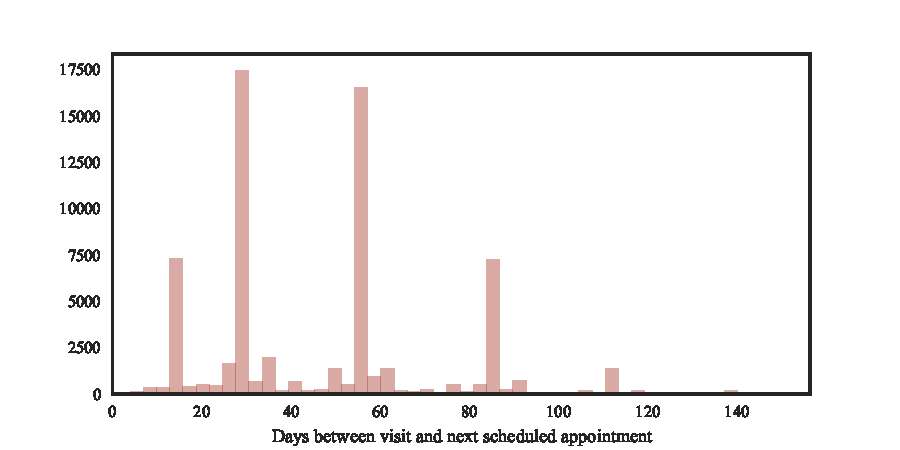
\includegraphics[width=\textwidth]{figure/time_to_appointment.pdf}
\caption{Distribution of $f_v^i$ in our data. We see the visits are scheduled mainly 7, 28, 56 or 84 days after the previous visit}
\label{fig:schedule_days}
\end{figure}
\end{center}

We can finally express the time between two visits as :
$$V_{v+1}^i - V_v^i = f_v^i + l_v^i  $$

\subsubsection{Data Entry}

The date at which a visit is recorded in an \gls{emr} database is $R(V_v^i)$. By definition, $R(V_v^i) \geq V_v^i$, and the delay in data entry is noted :
$$R(V_v^i) - V_v^i = \delta_v^i \geq 0$$

$\delta$ may vary in a facility, depending on the workload, staffing or other factors. In some cases, the visit has not and will never be recorded. I will note this situation as $\delta \rightarrow \infty$. Figure \ref{fig:data_entry_time} shows the distribution of $\delta$ in our data.

\begin{center}
\begin{figure}[ht]
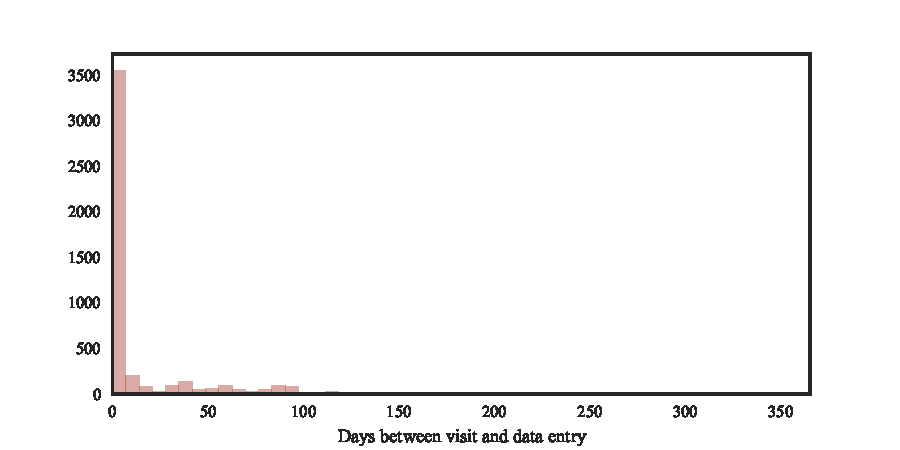
\includegraphics[width=\textwidth]{figure/data_entry_time.pdf}
\caption{Distribution of $\delta_v^i$ in our data. Most of the data is entered in the first week following the visit, but we see some data can be entered much later}
\label{fig:data_entry_time}
\end{figure}
\end{center}

Finally, data entry is interrupted at date $T_{close}$ before the data is used for analysis. The time elapsed between patient $i$'s last visit and the closing date is noted as $G_i = T_{close} - \max_v(A_v^i)$. For simplicity, we will equate the date of database closure with the date of analysis in a first step, and will relax this assumption when we will be measuring data maturity.


\pgfdeclarelayer{background}
\pgfdeclarelayer{foreground}
\pgfsetlayers{background,main,foreground}
\begin{center}
 \begin {figure}[ht]
        \centering
\resizebox{\linewidth} {!} {
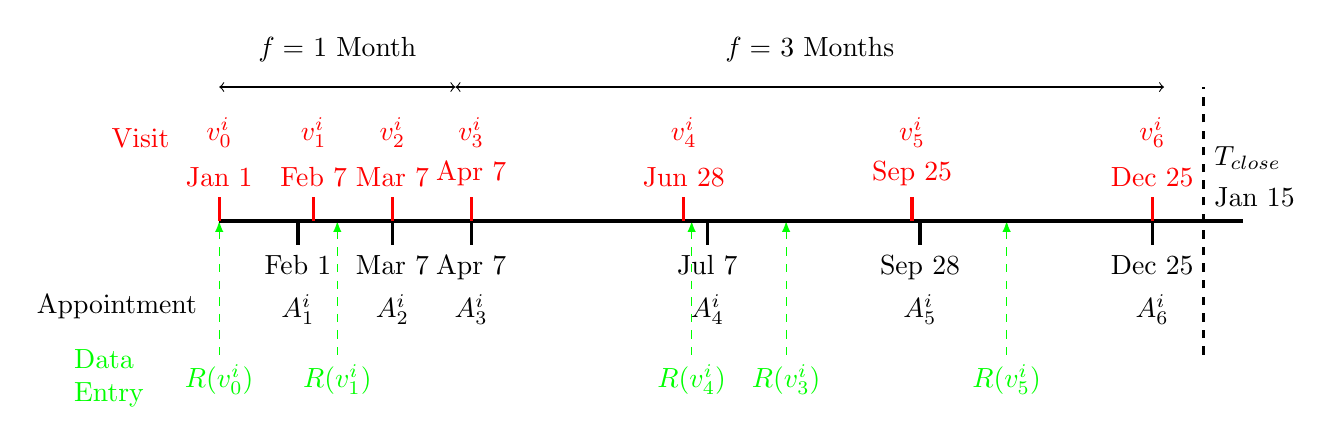
\begin{tikzpicture}


  \draw[<->] (0,1.7) -- (3,1.7);
  \draw[] (1.5,1.9) node[above]{$f =$ 1 Month};
  \draw[<->] (3,1.7) -- (12,1.7);
  \draw[] (7.5,1.9) node[above]{$f =$ 3 Months};


  \draw[ very thick] (0,0) -- (13,0);

\begin{pgfonlayer}{main}
  %% Draw Appointments
  \draw[very thick] (-1.3,-8mm)node[below]{Appointment};
  \foreach \x/\y/\z in {1/Feb 1/$A_1^i$,
                     2.2/Mar 7/$A_2^i$,
                     3.2/Apr 7/$A_3^i$,
                     6.2/Jul 7/$A_4^i$,
                     8.9/Sep 28/$A_5^i$,
                     11.85/Dec 25/$A_6^i$
                     }{
 \draw[very thick] (\x, 0) --+ (0,-3mm) node[below](\x){\fontsize{20}{22.4}\y}(\x,-8mm)node[below]{\z};
 }


  %% Draw Visits
  \draw[red , very thick] (-1,8mm)node[above]{Visit};
  \foreach \x/\y/\z in {0/Jan 1/$v_0^i$ ,
                     	1.2/Feb 7/$v_1^i$,
                     	2.2/Mar 7/$v_2^i$,
                     	3.2/Apr 7/$v_3^i$,
                     	5.9/Jun 28/$v_4^i$,
                     	8.8/Sep 25/$v_5^i$,
						11.85/Dec 25/$v_6^i$
                        }{
	\draw[red , very thick] (\x, 0) --+ (0,3mm) node[above](\x){\fontsize{20}{22.4}\y}(\x,8mm)node[above]{\z};
    }
\end{pgfonlayer}

\begin{pgfonlayer}{background}
    %% Draw Data Entry
    \draw[very thick ,  green] (-1.4,-25mm)node[above , align=left]{Data\\Entry};
    \foreach \x/\y in {0/$R(v_0^i)$,
  					   1.5/$R(v_1^i)$,
					   6/$R(v_4^i)$,
                       7.2/$R(v_3^i)$,
                       10/$R(v_5^i)$
                        }{
    \draw[dashed ,  green , latex-] (\x,0mm) -- +(0,-17mm)node[below]{\y};
    }

\draw[dashed ,  very thick] (12.5,-17mm) -- (12.5,17mm) ;
\draw[very thick] (12.5, 8mm)node[right]{$T_{close}$};
\draw[very thick] (12.5, 3mm)node[right]{Jan 15};

\end{pgfonlayer}

\end{tikzpicture}

}
\caption{Individual follow-up and data entry process}
\label{fig:timeline-followup}
\end{figure}
\end{center}

Figure \ref{fig:timeline-followup} shows how these different parameters can play out for a given patient. This imaginary patient had a first visit on January 1st, and had an appointment scheduled on February 1st, to which he came 6 days late. After three months of being seen monthly, he switched to a quarterly follow up. He was early to his July appointment, but came to every appointment until the end of the year. The data was entered very quick at the beginning of the year, but $v_2^i$ was never recorded. $v_4^i$ was entered before $v_3^i$, and $v_6^i$ could not be entered before the database was freezed for analysis on January 15 of the following year. This example gives a rough demonstration of the different situations and problems that can be encountered when analyzing the follow-up of the patient.

\subsubsection{Loss to Follow Up definition}

A central piece of the \gls{ltfu} definition is the  \textit{grace period} during which a patient, even if he did not return to a facility, is considered actively followed. This \textit{grace period} is denoted $G_0$.

A patient $i$ is considered \gls{ltfu} if he is late to his latest scheduled appointment for more than $G_0$ days.

$$l_{v^{*}}^i >  G_0$$

Looking closer at this definition, we can see it regroups three different situations :
\begin{enumerate}
\item $l_{v^{*}}^i \rightarrow \infty$ : The patient is \gls{ltfu} and will never come back to the facility.
\item $\infty > l_{v^{*},i} > G_0$ : The patient is late to his appointment but will come back in the future.
\item  $\delta_{v^*+1} > G_0$ : The patient came for his visit $v^{*} + 1$ but data entry took longer than the grace period and the visit was not entered at the time of database closure.
\end{enumerate}

Using this definition, we can express the probability that a patient is identified as \gls{ltfu} based on the data at hand. Let's $X = 1$ be the event that a patient is actively in care, and $X = 0$  the event that the patient is \gls{ltfu}. We can get $p(X = 0 | l_{v^{*}}^i \leq  G_0)$ as the combination of elements we can measure :

$$p(X = 0 | l_{v^{*}}^i >  G_0) = 1 - p(\infty > l_{v^{*}}^i >  G_0) - p(\delta_{v^*+1} > G_0) $$

We can understand $\infty > l_{v^{*}}^i \leq  G_0$ as an intrinsic myopia of the health system, who can not predict the future, and $\delta_{v^*+1} > G_0$ as a data quality measure. Differentiating between these two terms is  important in order to understand uncertainty in the \gls{ltfu} rate and better measure retention in the cohort.

\subsection{Data}

The data used for this aim are \gls{emr} database obtained from the HIV programs. I currently work with an \gls{emr} from  Kenya, and part of IHME's ABCE study. In this facility, 4833 patients have been registered for HIV care, from 2005 to June 2012, totaling 69591 recorded visits. Data entry time is easily available for at least 4853 of these visits.

I hope to obtain two additional \gls{emr} databases. The ISanté EMR, used in Haïti, and multiple implementations of the FUCHIA system, developped by Médecin Sans Frontières and used by the national HIV program in Niger. This would allow me to better measure variability in appointments lags and data entry issues. All the data will be analyzed anonymously and in aggregate form. For each patient, I only use visit dates and scheduled appointment dates. If scheduled appointment dates are missing, they will be imputed using observed $f^i_v$ in the data. I will also use the metadata collected in the EMR, especially the dates of data saving, to estimate data quality by measuring $\delta$ distribution.

I will not report precise data on HIV programs performance, and all the data used will be used to inform the simulation model.

\subsection{Methods}

This work will be done in three main steps. First, I will estimate the relevant quantities from the data at hand. In a second step, I will simulate a cohort and its monitoring, using estimated quantities as parameters. Finally, I will use this simulation, varying different parameters, to answer my main questions of interest.

\paragraph{Modeling -} The different parameters described earlier will be modeled and estimated  from the cohort data I will have at hand, using a Bayesian approach. The two most important parameters for this work are $\delta$, the time before visit has been recorded in a database, and $l$, the time between an appointment and the actual visit.

A first approach to modeling these parameters is to express $\delta$ as a Gamma distribution $\mathrm{G}(\alpha , \beta)$, with mean $\frac{\alpha}{\beta}$ representing the mean time to data entry of a visit form in the \gls{emr}. A Gamma distribution allows for a very long tail on the right, which will allow us to include data loss ($\delta  \rightarrow  \infty$).

$l$ could be modeled using a mixture model, to take into account the multimodal nature of the $l$. I will also have to consider the hypothesis that the multimodal $l$ distribution results from unrecorded shorter term appointments, and if this is the case we may need to use a long tailed distribution as for $\delta$.

\paragraph{Simulation - } Using the parameters estimated in the previous step, I will simulate an HIV patients cohort. This simulation will be made using the \gls{ceam} framework developed at IHME to simulate epidemiological cohorts, in which I will feed draws from the posterior distributions of the previously estimated models.

In a second step, I will simulate the data entry process, for any given month, by drawing a $\delta$ for each visit that will have been generated (initial or returning), and then computing the date of data entry for the information related to this visit.

As a result of this simulation, I will have all the information needed to estimate retention and measure of retention for the cohort. Finally, varying the relevant parameters, I will be able to measure the quantities of interest for my study aims.

\paragraph{Quantities of interest -} This simulated data will then be used to estimate our elements of interest :

\begin{enumerate}
\item \textbf{Measuring data quality impact} : From the cohort simulations, I will measure the LTFU rate using different distributions  of $\delta$. Different scenarios will be considered for data quality, varying both the mean and variance of $\delta$. Perfect data quality will be compared to situations with long delays of data entry, and situations with important data loss (high variance of $\delta$). The resulting observed variation in the \gls{ltfu} rate  will be described as the impact of data quality on the measure of retention.

\item \textbf{Data maturity} As data is being entered in the \gls{emr}, or as missed visits are finally being made, the data for a given period will get completed, and patients actively on care are more and more considered so. As data maturity grows in the  \gls{emr}, the data quality induced error is lowered. Varying $T_{close}$ can thus have an impact on the measure of retention of a patient on a given date. I will carry out the measure of retention using different closing dates for the database, and only using the data recorded before the closing date. These measures will allow me to define and test a Data Maturity metric, based on a combination of $f$, $l$ and $\delta$ that will allow us to identify the optimal minimum date of analysis to estimate retention rates in a program, and the optimal grace period $G_0$ to use for different levels of maturity.

\item{Robust measures of retention} Finally, we will consider more robust metrics that can be considered good proxies for retention. These metrics will include :
\begin{itemize}
	\item The ratio of the corrected average number of registered visits on the expected number of followed patients
	\item The ratio of new to returning patients in the facility
	\item The probability that the rate of \gls{ltfu} is higher than a given threshold
\end{itemize}
\end{enumerate}

For each of these metrics, I will evaluate their capacity to measure retention in the cohort, by comparing with the reference measure of \gls{ltfu}  measured with perfect data. I will also evaluate the sensibility of these metrics to data quality and data maturity.

\subsection{Timeline}
\label{timeline:aim1}

I have obtained the data I need for this aim and have made a first set of microsimulation and started the estimation of relevant parameters in my data. Based on this simulation, I will estimate data quality impact, data maturity impact and I will test robust measures of retention during the last quarter of 2017 and the first quarter of 2018, and I plan on having final results by March 2018. Figure \ref{GanttPaper1} summaries this timeline.

\begin{figure}[!t]
	\begin{ganttchart}[vgrid,hgrid,y unit chart=.6cm]{1}{9}
    \gantttitle{2017}{3}
    \gantttitle{2018}{6} \\
    \gantttitlelist{10,...,12}{1} \gantttitlelist{1,...,6}{1}\\

		\ganttset{bar/.append style={draw=red!40 , fill=red!40},
					group/.append style={draw=red, fill=red}}
		\ganttbar{Modeling and Model estimation}{1}{2} \\
		\ganttbar{Cohort Simulation}{1}{2} \\
		\ganttmilestone{Sharing Cohort simulation results}{2} \\
		\ganttbar{Data Quality Impact}{3}{3} \\
		\ganttbar{Data Maturity}{4}{5} \\
		\ganttbar{Robust Measures of retention}{4}{5} \\
		\ganttmilestone{Sharing Final Results}{6} \\
		\ganttbar{Paper Writing}{6}{8} \\
	\end{ganttchart}
	\caption{Gantt Chart for Aim 1}
	\label{GanttPaper1}
\end{figure}
